\documentclass{article}
\usepackage{graphicx}
\usepackage{hyperref}
\usepackage{fancyvrb}
\hypersetup{colorlinks,urlcolor=red}
\usepackage[margin=1in]{geometry}
\usepackage{listing}

\usepackage{amsmath}
\usepackage{amssymb}
\usepackage{amsthm}
\usepackage{mathtools} %for use of := symbol mostly.
\usepackage{booktabs} % used for making tables

\usepackage[export]{adjustbox} % allows frame around figure

\usepackage[round]{natbib}


\newcommand{\pnote}[1]{{\langle \text{#1} \rangle}}

\begin{document}

\title{TrawlExpert: Tool for Watershed Biological Research}
\author{Lab section: L01 \\ Christopher W. Schankula \\Student ID: 400026650 \\schankuc@mcmaster.ca}

\maketitle

\section{Objective}
Statistical and visual tool for the analysis of water ecosystems, based on scientific water trawl data. Provides researchers with tools to analyze large datasets to find patterns in fish populations, including the plotting of historical population data on a map, analyzing population trends over time and finding subpopulations of a certain species, genus, family, etc.

\section{Motivation}
The diminishing of fish populations in the Great Lakes became a problem in the latter half of the 20th century, with the total prey fish biomass declining in Lakes Superior, Michigan, Huron and Ontario between 1978 and 2015 \citep{michigan2017}. Annual bottom trawl surveys involve using specialized equipment to sweep an area and are used to determine the relative temporal variation in stock size, mortality and birth rates of different fish species \citep{walsh1997efficiency}. These surveys are performed annually and often have hundreds of thousands of records, making manual analysis infeasible. The ongoing protection and development of the Great Lakes water basins is considered an important topic for scientists in both Canada and the United States, as evidenced by grants such as the \textit{Michigan Sea Grant} \citep{michseagr2018}.

TrawlExpert will give researchers tools to filter through these large amounts of data by allowing them to search through data based on class, order, genus, family or species. This will help support scientific researchers and fishing companies as they study fish populations in order to launch initiatives to preserve fish populations and perform their business in an environmentally friendly way going forward. As more data is collected on an annual basis, TrawlExpert can easily be injected with the new data and will adjust and scale accordingly, combining the new data with the old data for continued analysis.

TrawlExpert will also analyze the trawl data to find connected subpopulations within the data, giving researchers  tools to analyze the portions of the water body that contain different populations and even track these specific subpopulations over time.

The focus of the project will be to develop these unique data searching and querying tools as a first step in a complete trawl survey analysis. For a complete analysis, tools like stratified statistical analysis would be required by the researcher \citep{walsh1997efficiency}. For purposes of maintaining a scope for this project, the implementation of advanced trawl survey scientific and statistical analysis tools will be relegated to future developments. 

\section{Prior Work}
From preliminary research, past software has been developed to analyze trawl survey data. One such piece of software is MIXFISH which is part of the LFSA package written in BASIC in 1987 \citep{sparre1987computer}. MIXFISH / LFSA has been used by several researchers, (e.g. \cite{levi1993analysis}, \cite{chakraborty1996stock}), while performing trawl survey analyses. Most of these were confined to running on smaller samples of data (e.g. 1000 samples for a given species); however, with modern hardware and using a modern programming language, TrawlExpert will allow processing of much larger datasets.

Other studies, e.g \cite{swartzman1992spatial}, make use of software programs to perform statistical analysis but do not use software specialized to analyzing trawl survey data. Although the main focus of this semester's project will be the searching and selection of data, TrawlExpert's goal will be to give researchers an all-in-one platform in order to perform their analysis, in each step of the analysis pipeline.

\section{Input / Output and Proposed Solutions}
\subsection{Datasets}\label{sec:out}
The test dataset that will be used for purposes of this project is the \textit{USGS Great Lakes Science Center Research Vessel Catch Information System Trawl} published by the United States Geological Survey. Compiled on yearly operations taking place from early spring to late fall from 1958 until 2016, the dataset contains over 283,000 trawl occurrences in the five Great Lakes, including the latitude and longitude co-ordinates and biological classification such as family, genus and species. A complementary dataset contains 45,000 entries detailing the operations and parameters such as equipment.

\subsection{Outputs}

This section describes in detail the types of data analysis and queries that TrawlExpert will be able to perform. Section \ref{sec:case} describes a potential use case for a researcher studying a body of water.

\subsubsection{Output 1: Historical Distribution}
Researchers will be able to query for historical population data of a certain genus, family, etc, outputted in text format or generated as a figure.

\subsubsection{Output 2: Geographical Distribution}
For a given species over a given timeframe, the program will output the locations of all records matching that query in terms of the recorded location at which the fish were found.

\subsubsection{Output 3: Geographical Subgroupings}\label{sec:subgroup}
The third main type of output will be to classify a given search into subgroupings of highly clustered populations (see section \ref{sec:graphalgs} and figure \ref{fig:Groupings}).

\subsection{Family Subgroupings: A Use Case Example}\label{sec:case}
The dataset presented in section \ref{sec:out} will be used as the main input in order to generate these outputs. The location and temporal data given in the dataset will be used to help generate outputs 1 and 2. In order to illustrate this, the following example use case will be presented and analyzed:

A researcher is studying the decline of all species in the family \textit{Cyprinidae}. She has a large dataset of trawl data and wishes to obtain information about the related subpopulations in the data. Therefore, she uses the TrawlExpert to generate an output of type 3 which will give her the output she needs for her research. By recursing down a pre-built tree structure built from the data (described in more detail in section \ref{sec:graphalgs}), the program will determine which genera, species and potentially subspecies are included in this family of organisms. It will locate all entries for this expanded search. These entries each contain the latitude and longitude at which the sightings were made. The program will then cluster geographically close results and return a list of these subgroupings, either in text format or visualized as a figure.

The researcher can now continue her scientific analysis of the data having easily and intelligently narrowed down to relevant data.

\section{Algorithmic Challenges}
\subsection{Searching Algorithms}
A modified form of binary search will be used for quickly locating the first of a given key in the large dataset and will be a crucial building block of all three main types of output. This will allow all entries of that type to be found to the right of that result.

\subsection{Sorting Algorithms}
Sorting will be crucial for both ordering historical data in chronological order as well as being the basis for binary search to work, since it requires data to be sorted. The mergesort algorithm will be advantageous due to its fast and predictable runtime ($N\lg N$).

\subsection{Graph Algorithms}\label{sec:graphalgs}
Graph algorithms will be used for the advanced searching features of the program. Firstly, the biological classification of each organism forms a tree from which species in the same genus, for example, can be located. Secondly, a graph algorithm will be used to find connected components for generating output of type 3 described in section \ref{sec:subgroup}. Entries form nodes which can be connected together based on their distance to surrounding points and a breadth-first search algorithm will be used to determine connected components \citep{broder2000graph}. This is visualized in figure \ref{fig:Groupings}.

\begin{figure*}[t]
\centering
\begin{tabular}{ p{32mm}p{32mm}p{32mm}p{32mm} }
a) & b) & c) & d)\\
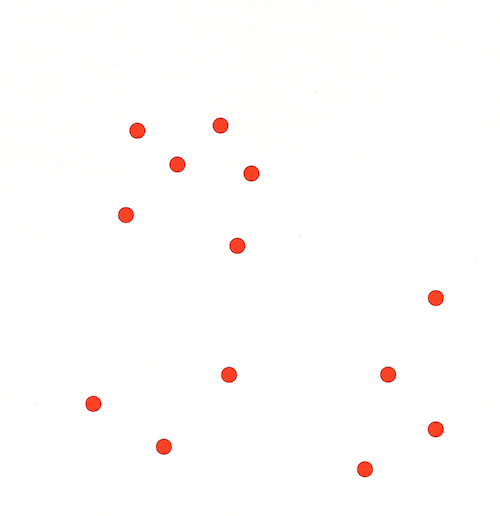
\includegraphics[width=35mm,frame=0.01cm]{Fig.png} & 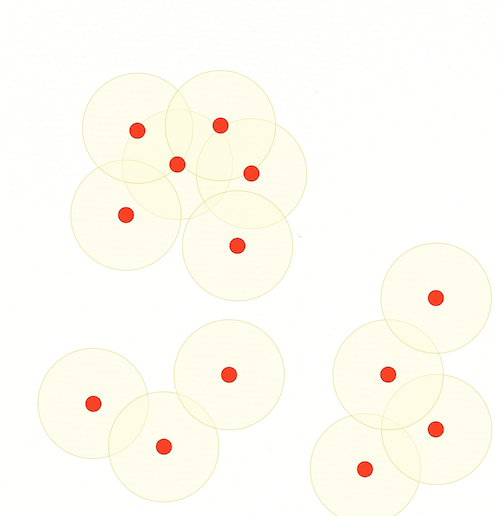
\includegraphics[width=35mm,frame=0.01cm]{Fig2.png} & 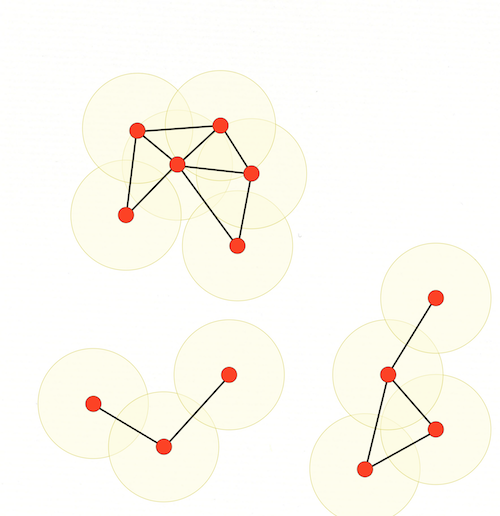
\includegraphics[width=35mm,frame=0.01cm]{Fig3.png} & 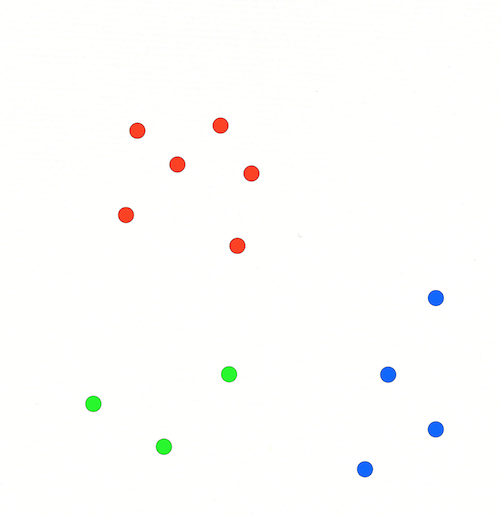
\includegraphics[width=35mm,frame=0.01cm]{Fig4.png}
\end{tabular}
\caption{A visualization of the proposed algorithm for output 3. In a), there are some species sightings that the user wishes to group. In b), a radius of similarity is chosen by the user. In c), overlapping regions determine connected points, creating a graph structure with groups of connected points. In d), the points are classified into groups by finding connected components of the graph structure. }
\label{fig:Groupings}
\end{figure*}

\clearpage
\section{Project Plan}
The following milestones will help inform our progress towards completing the goals. The team should be divided up into two subteams for maximum efficiency:

\begin{table}[h]
	\centering
	\begin{tabular}{p{0.16\hsize}p{0.38\hsize}p{0.38\hsize}}
		\toprule
		\textbf{Milestone} & \textbf{Subteam A} & \textbf{Subteam B}\\
		\midrule
		Milestone 1 \newline (``Bedrock'') \newline(End of Week 1)
		& Finished parsing module for .csv data to create Java objects that can be used for analysis; start data cleansing
		& General binary search module underway \\
		\midrule
		Milestone 2 \newline (``Quartz'') \newline(End of Week 2)
		& Cleansed the data to remove or correct entries not containing all of the columns; start generating biological classification tree module
		& Finished and tested binary search; start mergesort \\
		\midrule
		Milestone 3 \newline (``Granite'') \newline(End of Week 4)
		& Finished and tested classification tree; start data visualization or formatted text output tools
		& Finished and tested mergesort; start writing query module for output type 1 and 2, using mergesort and binary search to get results from data \\
		\midrule
		Milestone 4 \newline (``Sandstone'') \newline(End of Week 6)
		& Continue data visualization or text output tools; start helping subteam B if needed
		& Continue query module: finished output 1 \& 2; start output type 3\\
		\midrule
		Milestone 5 \newline (``Diamond'') \newline(End of Week 8)
		& Finished data visualization or text output tools; start using them to display outputs; work on keynote presentation
		& Finished output type 3; work on keynote presentation \\		
		\bottomrule
	\end{tabular}
\end{table}

While this schedule provides a good reference and a way to monitor progress, it may have to be modified throughout. For example, if a milestone is reached before its given date, the next milestone should start development early. Approximately 1-2 weeks has been purposely left as padding at the end in case of unforeseen circumstances.

\clearpage
\bibliographystyle{apa}
\bibliography{bib}

\end{document}